\chapter{Introduction} \label{introduction} 

The purpose of this research is to contribute in the diverse forms of use of the interactive learning environments by proposing a learning environment, we based the content management with an adaptive hypermedia approach and 
with the development of a new type of learning object to be adapted to the learning environment.
This environment use various devices that were capable of running a web browser, non-relational data bases for information exchange and some sensors like cameras and Kinect 2 were used. In addition we implemented a way to predict the level of user attention
which it was compared against information obtained by a video taken from the user doing the activity.

\section{Motivation}
There are many types of learning environments starting from the most basic that exist almost from the beginning of civilization where a person is able to learn based on their current context.
For example the first humans who needed to hunt them could take decisions and adapt to the situation and perform the task that was to hunt an animal to obtain food, in more recent times we can relate to the classrooms of schools, and currently including technology these Environments can be configurable and adapt to a particular context (the user).When a user uses learning environments the themes are usually flat and have the same content for everyone. In addition, users think and assimilate information in a different way which makes it more attractive to have a learning environment that adapts to the learning styles of the users and why not to the user preferences.

Nowadays most interactive museums work stations or exhibits like we see on the figure 1.1, where users come to the station to interact with or receive information by reversing some time on it until it passes to the next station, where the display will probably showed relevant information for the person but if this information is not shown to digestible way (processed so that it is attractive to the user) the user will probably spend less time or not time at all at the station. This expose the lack of adaptation of the exhibits in some interactive museums or standard museums. in order to ensure that the information and how is presented to the user is broadly engaging. 
\begin{figure}[ht!]  
\centering  
\includegraphics[scale=0.05]{musint}
\quad  
\caption{A museum interactive station}  
\label{name}  
\end{figure}
Intelligent learning environments can be used as exhibitors in museums they use embedded systems, sensors, information and communication technologies that are becoming invisible to the user as they are being integrated into physical objects, infrastructure, the environment in which we live, work and many other environments. This idea provides a good way of bridging the gap between human users and computing systems, and this motivates related research into Computing. Some of these systems use learning resources called learning objects. For the ex-change of learning objects between systems standardization initiatives have been developed and there are some implementations and repositories that manage the content using these standards. 

\section{Learning Environment}
Learning environment refers to the diverse physical locations, contexts, and cultures in which students learn. Since students may learn in a wide variety of settings, such as outside-of-school locations and outdoor environments, the term is often used as a more accurate or preferred alternative to classroom, which has more limited and traditional connotations—a room with rows of desks and a chalkboard, for example.
The term also encompasses the culture of a school or class—its presiding ethos and characteristics, including how individuals interact with and treat one another—as well as the ways in which teachers may organize an educational setting to facilitate learning—e.g., by conducting classes in relevant natural ecosystems, grouping desks in specific ways, decorating the walls with learning materials, or utilizing audio, visual, and digital technologies. And because the qualities and characteristics of a learning environment are determined by a wide variety of factors, school policies, governance structures, and other features may also be considered elements of a “learning environment”.

Educators may also argue that learning environments have both a direct and indirect influence on student learning, including their engagement in what is being taught, their motivation to learn, and their sense of well-being, belonging, and personal safety. For example, learning environments filled with sunlight and stimulating educational materials would likely be considered more conducive to learning than drab spaces without windows or decoration, as would schools with fewer incidences of misbehavior, disorder, bullying, and illegal activity. How adults interact with students and how students interact with one another may also be considered aspects of a learning environment, and phrases such as “positive learning environment” or “negative learning environment” are commonly used in reference to the social and emotional dimensions of a school or class.

The Learning Environment (LE) corresponds to the spaces in which the learning activities are developed, can be of three types: aulic, real and virtual. In the first it is the whole environment surrounding the student, in the context of the classroom, which focuses not only on the student, but also on the content, so the interaction with the environment will develop an interaction with the student that can be positive or negative depending the place. And has the following characteristics: 
\begin{itemize}
 \item The educator is the one who has to look for the models appropriate to their materials and the conditions of their group.
 \item They help to relate the content in an experimental and experiential way.
 \item It can be given a dynamic spatial distribution, changing as the group and the teacher consider it necessary.
\end{itemize}

The real Teaching-Learning activities are developed in the classroom, the real environment can be a laboratory, a company, clinic, library, green areas, etc. Real scenarios where you can see the application of knowledge and skills acquired, as well as the practice of attitudes and values. 

Virtual environments are those created through the use of Information and Communication Technologies, in order to provide learners with resources that facilitate their learning process, within these TICs can be cited the computer, cannon, a classroom Virtual, the use of internet where they can have access to blogs, discussion forums, chat, specialized pages where young people find fun activities, stories like solution to crosswords, puzzles, etc., that well employees contribute greatly in:
\begin{itemize}	
\item Acquisition of learning by the student.
\item Understand the nature and philosophy of distance education.
\item Identify the characteristics of students in remote locations.
\item Design and develop interactive materials that are adapted to the technology to be used, to the content, strategies and to facilitate independent study.
\end{itemize}
Learning environments are important in the day-to-day lives of people because we are in contact with them all the time in accordance with Phillips\citep{PhilMcNaKenn2010zx} a Learning Environment is a place where resources, time and reasons are available for a group of people to nurture, support and value the learning of a limited set of information. The LE are social places even when only one person is found there. 



One of the challenges facing the design of learning environments is human complexity, because each person thinks and assimilate information in different ways making it difficult to identify which resources are adequate for everyone. Intelligent learning environments (ILE) are a new type of intelligent educational system, which combines characteristics of traditional intelligent tutoring systems (ITS) \citep{john1991} and learning environments. According to Self \cite{self1998} ITS are learning systems based on computers that try to adapt to the needs of the learner. 
\begin{figure}[ht!]  
\centering  
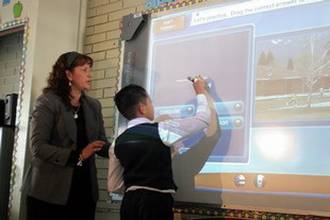
\includegraphics[scale=1]{pizzarra}
\quad  
\caption{A kid using and intelligent chalk-board}  
\label{name}  
\end{figure}

According to the literature, providing effective support or guidance by identifying the knowledge levels and learning difficulties of students in learning programming languages could be the key to the improvement in students’ learning performance. Researchers have indicated the important role of assessment in identifying the learning status of individual students in providing effective learning guidance \cite{HWANG2003217} \cite{BJET1319} \cite{TSENG2008776}. Researchers have further argued that assessment could be used as a learning strategy to improve students’ learning performance \cite{CHU20101618} \cite{GALVEZ2009279} . For example, Hauswirth and Adamoli \cite{HAUSWIRTH2013499} proposed a pedagogical approach aligned with this aspect that allows students to learn from their mistakes by answering a series of questions. On the other hand, researchers have also indicated that assessing students’ programming knowledge and skills as well as identifying their learning difficulties remains a challenging issue, implying the need to develop effective strategies or tools to identify students’ status and provide learning support in programming language courses \cite{WANG2012412}.   
 
In the past decade, various teaching strategies and learning activities have been applied to computer-programming courses for beginners \cite{GOVENDER20091218}. For example, Machanick \cite{MACHANICK2007396} proposed the idea of abstraction-first teaching by hiding details until students are ready for them. In addition, Emurian, Holden, and Abarbanel \cite{EMURIAN2008576} employed a peer-tutoring approach, and Hwang, Shadiev, Wang, and Huang \cite{HWANG20121267} proposed a web-based programming-assisted system to provide learning support for programming courses. In the meantime, researchers have indicated that problem-based learning (PBL) could be a promising approach for programming language learning \cite{KORDAKI201069}. For example, Gálvez, Guzmán, and Conejo \cite{GALVEZ2009279} reported a problem-solving environment to diagnose students’ knowledge levels and to generate feedback and hints to help students understand and overcome their misconceptions in learning programming languages. 


\section{Learnign Objects.}
A Learning object is defined by Wayne Hodgins \cite{wayneh} as "a collection of content items, practice items, and assessment items that are combined based on a single learning objective". When he created a working group in 1994 though the concept was first described by Gerard in 1967 \cite{gerard1967}. Learning objects go by many names, including content objects, educational objects, information objects, intelligent objects, knowledge bits, knowledge objects, learning components, media objects, reusable curriculum components, nuggets, reusable information objects, reusable learning objects, testable reusable units of cognition, training components, and units of learning. The Institute of Electrical and Electronics Engineers (IEEE) \cite{ieee} defines a learning object as "any entity, digital or non-digital, that may be used for learning, education or training", Chiappe \cite{ChiappeLaverde2007} defined Learning Objects as: "A digital self-contained and reusable entity, with a clear educational purpose, with at least three internal and editable components: content, learning activities and elements of context. The learning objects must have an external structure of information to facilitate their identification, storage and retrieval: the metadata.".
 Learning Objects and Metadata Based on the object-oriented paradigm, learning objects are typically defined as components of instruction material, which can be reused in multiple contexts. Instruction designers can create and maintain these components, independent of each other and share them over the Internet \cite{Dattolo2000}. 

Since many studies generated about in recent years, some authors organize these objects at different levels, regardless of the many groups that, according to the fields of descriptors, we could set up. In the case of structuring levels, the first one would refer to the tiniest units that could be assigned the name of learning objects: a digital image (graphic, photo, diagram, map, chart, ... ), a table, phrase, or sound formula (bell, telephone, storm, animal, ...), etc. The following levels are assuming units increasingly complex and, logically, less adaptable to other contexts or learning contents. According to the fields, areas of knowledge, dimensions or other taxonomic forms, the organization of objects can take many forms. For this organization, these objects, in addition to their reuse characteristics, must have the possibility of being updated, combined, separated, referenced and systematized. In this way, they are classified or cataloged and labeled to be located in the corresponding warehouses or repositories of contents or objects, so that later they can be located for reuse or, if necessary, modification or re-elaboration, through the corresponding contrast, comparison strategies , Relationship and criticism of the information obtained. That is why it obviates the need for powerful learning object repositories. Hence, the object and the repository are two complementary entities. An object that does not have the necessary characteristics to be able to integrate in a repository, loses all its virtualities and, at the same time, a repository that does not have a good base of objects, stops being interesting and operative. There are institutional repositories, training companies, associations, consortium, organizations, etc. The Web itself could be considered as a large repository, provided that we apply the strategies of search, processing, selection and cataloging through metadata schemes. The metadata structure implies having a detailed textual structure, describing attributes, properties and characteristics distributed in different fields that clearly identify the object, so that it can be found, assembled, and used. 

Asi que es muy importante para los ambientes de aprendizaje contar con una buena administracion y dustribucion de objetos de aprendizaje 


\section{Aim's.}

Learning environments have been extensively used physically, virtual and for various purposes such as training, entertainment, demonstration, etc.
But the problem remains of how to present the information, more specifically how to adapt the content to the user or users of these environments.
Using new technologies improves these environments by allowing them to display information across devices by labeling them as learning objects, a good set of learning objects displayed can enhance learning against traditional learning \cite{Chen2007}.


The aim of this thesis is to create an adaptive learning environment, reduce implementation costs of the learning environment using any device compatible with a web browser,
define new type of learning object that we call Environmental learning object, develop a learning environment that can use devices that do not require special installation and are compatible between themselves and the environment. Using e-learnign combined with the simple sequencing standard, learning objects, sensors to analyze if the user likes what they are observing and a technique to distribute the learning objects in the environment and thus adapting the environment to the user in each of the activities performed in the environment until the sequence ends or decides to stop performing the activity. To achieve this, a learning sequence is established, which is previously configured based on the learning context, the user navigates through the sequence thanks to a fuzzy system that allows to semi-automate the course of the learning sequence or waiting for the User performs an action that affects the path of the sequence, at the same time a sensor that measures the level of attention of the user allowing to study and measure if the content shown is optimal for the user.

The contribution of this thesis is the new adaptive learning environment which includes a new type of learning object and a method to measure the level of attention of the user. It provides learning environments suitable for users. As an extra, this environment has characteristics that allow it to adapt to diverse contexts such as entertainment, advertising, museum exhibit, training, etc.
Several particular aims were done in order to support the achievement of contributions:

\begin{itemize}	
\item Elaborate an analysis about the state of the art in the field of intelligent learning environments and learning objects through the revision of the relevant literature. State of the art helps to define the tendency of currents intelligent learning environments, the recent improves and helps to understand what is the relevance of the proposed method as well as the feasibility and how we can make an important contribution to the intelligent learning environments.

\item  Design and conduct several experiments with the proposed LE. The experiments were based on experiments made by other similar methods. The metric implemented to measure the experiments results was compare each others and survey the users. 

\item  Selection of learning environments(including normal and intelligent LE) that are representative of the alternatives for this problem domain in order to compare their performance. There are not enough papers including all the problems attacked in this work to make a consensus about what is that we want from each one.

\item Propose an intelligent learning environment to use the new learning object and apply it in a case of study where the environment and the user are involved. 

\item Develop a prototype of an adaptive intelligent learning environment using the learning object proposed. Using several technologies to deploy the learning objects in the environment. This prototype lets users interact with the environment and allows us to analyze their behavior. 
   
\item To evaluate the proposed method we develop a method to evaluate the level of attention or engagement as it is called in literature of the users, using the environment. Results are explained in a posterior chapter.

\end{itemize}
\section{Outline.}
The rest of this thesis is organized as follows:
\begin{itemize}	
\item \textbf{Chapter 2}, 
describes a study and background of current and related work, presenting a general overview of learning environments and their improvement in recent years. This study includes intelligent learning environments, their classification, the technologies they use and their techniques. As well as the
challenges of these systems. The types of learning objects that exist as well as where and how they have been used and their contributions in the environments. Also the affective computation and how it affects the configuration of the learning environment. And finally describes the adaptive learning environments with an analysis of its advantages and disadvantages when using the adaptive techniques in interactive learning environments.

\item \textbf{Chapter 3}, 
describe the concepts that complement the bases of the method proposed in this thesis.

\item \textbf{Chapter 4}, presents the model of the adaptive learning environment, the proposed method involves the paradigm of configuring or contextualizing a learning environment adapting it to a user or group of users.
This chapter includes the overall explanation of data models and the functionality, as well as its components for this case of study.

\item \textbf{Chapter 5}, the results of the different experiments are presented. . This chapter also details the results
for each experiment from a point of view of scientific results.
\item \textbf{Chapter 6}, after the development of the learning environment, the impact of content in LE was evaluated. This chapter
describes the tests that were applied by surveys and sensors in order to evaluate the level of engagements of the users. Details of the environment and the characteristics of the
tests are described, as well as the results of each one. 
\item \textbf{Chapter 7}, this chapter concludes with a summary of its contributions and limitations. Final conclusions are drawn and also proposals for future work
are presented.

%At the end, this thesis includes appendices that describe detailed technical aspects about installation and libraries of python that uses the context-aware recommender system (appendix ??), the pseudocode of algorithms proposed in the method are available in (appendix ??), and experiment study materials used to obtain the test results are in (appendix ??).
\end{itemize}
